\newpage
\mysection{Scope}


Scope deals with where variables are "visible" in a program. There are many nuances when talking about scope so if you are looking for an in depth explanation on all the types of scope try this site: \href{https://en.cppreference.com/w/cpp/language/scope}{cppreference.com}. This section on scope is just a simple refresher of the most basic scoping rules.\\

What we usually deal with in class is \btic{block scope} or in other words \btic{global} and \btic{local} variables. Like the term implies (to me anyway), \btic{block scope} classifies variables declared within a block as \btic{local} to that block. Variables declared outside of any block are classified as \btic{global} variables. But as always, there are some nuances that are best explained using examples.

\mysubsection{Block}

First, what is a \btic{block}? A block is a pair of curly braces \btic{\textbf{\{\}}} used as an organizational construct to define the body of a function, class, method, loop, etc. but it also can be used outside of those constructs to simply define \btic{scope}. The example below multiples blocks nested within each other and not a function, loop, or if statement in site. Would this compile? Sure, if you added a few things. But it by itself is valid (OK there's one error, can you find it?). The question is, whats going with those nested blocks?

\begin{minted}[]{c++}
{
    int x = 1;
    cout << x << endl;            
    {
        cout << x << endl;        
        int x = 2;
        int y = 5;
        cout << x << endl;        
        {
            cout << x << endl;
            int x = 3;
            cout << x << endl;
        }
        cout << x << endl;
    }
    cout << x << endl;
    cout << y << endl;
}
\end{minted}

\textbf{Block Scope Rules:}
\begin{itemize}
    \tightlist
    \item Blocks are portions of code contained within curly braces \btic{\{....\} }.
    \item Identifiers declared within a block have block scope and are visible from their points of definition to the end of the innermost containing block.
    \item A duplicate identifier name in a block hides the value of an identifier with the same name defined outside the block.
    \item A variable name declared in a block is local to that block. It can be used only in it and the other blocks contained under it. 
\end{itemize}
  
\myheading{Example 1:}
\begin{itemize}
\tightlist
    \item This example has 3 code blocks, or 3 scope levels
    \item There is an \btic{x} declared at every scope level, so each \btic{cout} should reference the \btic{x} at its own level, \textbf{if the \btic{x} was declared before it was used.}
    \item If there is no variable declared within a code block before it is used, then it will use the value from the next level up. 
    \item If there is no variable declared in the previous level, it will continue to go up levels until it finds a variable with the same name, or error if one doesn't exist.
\end{itemize}

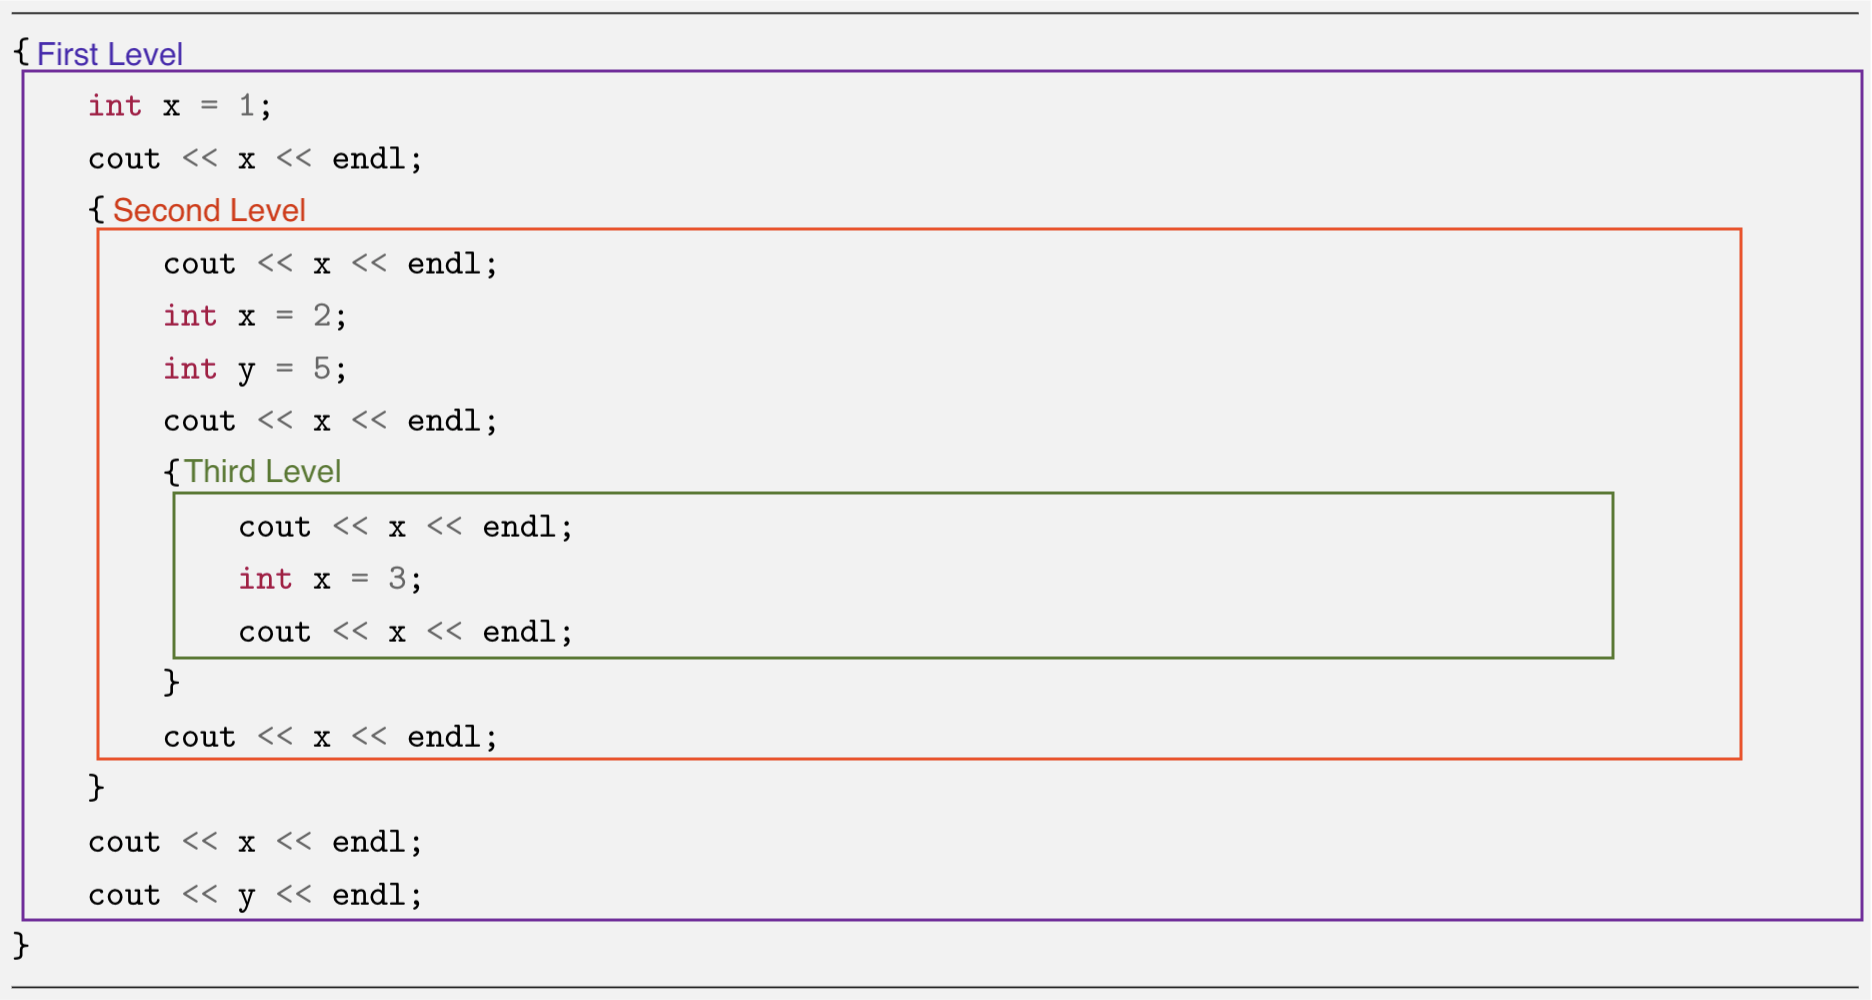
\includegraphics[width=6in]{images/scoping_rules.png}


\begin{minted}[linenos]{c++}
{
    int x = 1;
    cout << x << endl;          // OUTPUTS: 1 (uses level 1 x)
    {
        cout << x << endl;      // OUTPUTS: 1 (uses level 1 x)
        int x = 2;
        int y = 5;
        cout << x << endl;      // OUTPUTS: 2 (uses level 2 x)
        {
            cout << x << endl;  // OUTPUTS: 2 (uses level 2 x)
            int x = 3;
            cout << x << endl;  // OUTPUTS: 3 (uses level 3 x)
        }
        cout << x << endl;      // OUTPUTS: 2 (uses level 2 x) 
    }
    cout << x << endl;          // OUTPUTS: 1 (uses level 1 x)
    cout << y << endl;          // ERROR
}
\end{minted}

\myheading{Example 2:}

\begin{minted}[]{c++}
{
    int x = 1;
    int y = 2;
    cout << x << endl;          // OUTPUTS: 1 (uses level 1 x)
    {
        cout << x << endl;      // OUTPUTS: 1 (uses level 1 x)
        {
            int y = 4;
            cout << x << endl;  // OUTPUTS: 1 (uses level 1 x)
            cout << y << endl;  // OUTPUTS: 4 (uses level 3 y)
        }
        cout << x << endl;      // OUTPUTS: 1 (uses level 1 x)
    }
    cout << x << endl;          // OUTPUTS: 1 (uses level 1 x)
    cout << y << endl;          // OUTPUTS: 2 (uses level 1 y)
}
\end{minted}

\mysubsection{Local Variables}

Below we have a variable declared in the function \btic{someAge} 

\begin{minted}[]{c++}
/**
 * The variable age is local to this function.
 */
void someAge() {    
    int age=18;     
} 
 
/**
 * The variable age cannot be accessed from main
 */
int main() 
{ 
    cout<<"Age is: "<<age; 
    return 0; 
}
\end{minted}

\textbf{Output:}
\begin{minted}[bgcolor=bg]{text}
Error: age was not declared in this scope
\end{minted}

To get access to that local variable declared within that functions code block, you need to return it. 
\begin{minted}[]{c++}
/**
 * The variable age is local to this function.
 */
int someAge() {    
    int age=18;   
    
    return age;
} 
 
/**
 * Were still not accessing the variable from someAge()
 * we just got a copy of it. 
 */
int main() 
{ 
    cout<<"Age is: "<<someAge(); 
    return 0; 
}
\end{minted}

\textbf{Output:}
\begin{minted}[bgcolor=bg]{text}
Age is: 18
\end{minted}

\mysubsection{Global Variables}

\begin{itemize}
\tightlist
    \item Global variables are defined outside of all the functions, usually at the top of your program.
    \item They will hold their value throughout the life-time of your program.
    \item They can also be accessed by any function, unless a variable with the same name is declared within the functions code block. 
\end{itemize}
 

\begin{minted}[]{c++}
// Global variable declaration:
int g;
 
int main () {
   // Local variable declaration:
   int a, b;
 
   // actual initialization
   a = 10;
   b = 20;
   g = a + b;
  
   cout << g;
 
   return 0;
}
\end{minted}

\textbf{Output:}
\begin{minted}[bgcolor=bg]{text}
30
\end{minted}

\begin{minted}[]{c++}
// Global variable declaration:
int g = 20;
 
int main () {
   // Local variable declaration:
   int g = 10;
 
   cout << g;
 
   return 0;
}
\end{minted}

\textbf{Output:}
\begin{minted}[bgcolor=bg]{text}
10
\end{minted}